\chapter*{Introducción. Conexión por arcos}

Antes de comenzar con el contenido propio de la asignatura repasaremos algunos resultados que se estudiaron en Topología I pero que serán necesarios para el desarrollo de Topología II.

\section{Conexión}

\begin{notacion}
    Notaremos por e.t. al espacio topológico $(X,\cc{T})$ o diremos que $X$ es un e.t; puesto que la topología $\cc{T}$ se dará por conocida.

    Si $X$ fuese un subconjunto de $\bb{R}^n$, entonces, salvo que se especifique lo contrario, entenderemos que la topología asociada de $X$ es la topología usual $\cc{T}_u$ inducida.
\end{notacion}

\begin{definicion}
    Se dice que un e.t. $X$ es \textbf{no conexo} si existen $\emptyset \neq U, V$ abiertos en $X$ disjuntos y no vacíos tales que $X=U\cup V$ y $U\cap V = \emptyset$. 
\end{definicion}

\begin{prop}
    Dado un e.t. $X$ equivalen las siguientes afirmaciones:
    \begin{enumerate}
        \item[(i)] $X$ es conexo.
        \item[(ii)] Los únicos subconjuntos de $X$ que son abiertos y cerrados a la vez son el vacío y el total. 
        \item[(iii)] Los únicos subconjuntos de $X$ con frontera vacía son el vacío y el total. 
    \end{enumerate}
\end{prop}

\begin{definicion}
    Dado un e.t. $X$ y $A\subset X$, diremos que $A$ es \textbf{conexo} si $A$ es conexo con la topología inducida de $X$.
\end{definicion}

\begin{teo}
    La imagen mediante una aplicación continua de un conexo es conexa. Es decir, dado $f:X\to Y$ continua, si $X$ es conexo entonces $f(X)$ es conexo.
    
    En particular, ser conexo es una propiedad topológica (se conserva por homeomorfismos).
\end{teo}

\begin{teo}\label{teo:union_conexos}
    La unión de una colección de subconjuntos conexos que tienen un punto común de un e.t. $X$ es también conexa. Es decir, si $X$ es un e.t. y $\{A_i\}_{i\in I}$ es una familia de subconjuntos conexos de $X$ tal que $\bigcap\limits_{i\in I}A_i \neq \emptyset$, entonces $\bigcup\limits_{i\in I}A_i$ es conexo.
\end{teo}

\begin{teo}
    Si $A$ es un subconjunto del e.t. $X$ y $A$ es conexo, entonces dado $B$ con $A\subset B\subset\overline{A}$ se tiene que $B$ también es conexo. En particular, la adherencia de un conexo siempre es un conjunto conexo.
\end{teo}

\begin{teo}
    Dados dos espacios topológicos $X,Y$ se cumple que $X\times Y$ es conexo (con la topología producto) si y solo si $X$ e $Y$ son conexos.
\end{teo}

\begin{teo}
    Los conjuntos conexos de $\bb{R}$ con la topología usual son exactamente los intervalos (incluyendo los puntos).
\end{teo}

\begin{definicion}
    Dados un e.t. $X$ y un punto $x_0\in X$, se define la \textbf{componente conexa} de $x_0$ en $X$, notada por $C(x_0)$, como el mayor conexo de $X$ que contiene a $x_0$.
\end{definicion}

\begin{prop}
    Dadas un e.t. $X$ y un punto $x_0\in X$, la componente conexa de $x_0$, $C(x_0)$, es un conjunto conexo cerrado de $X$.
\end{prop}

\begin{teo}
    Las componentes conexas de un e.t. $X$ forman una partición de $X$ en conjuntos conexos maximales y cerrados.
\end{teo}

\section{Conexión por arcos}

Introducimos a continuación la conexión por arcos, que se trata de un concepto ligeramente más restrictivo.

\begin{definicion}
    Un \textbf{arco} (o camino) en un espacio topológico $X$ es una aplicación continua $\alpha:[0,1]\to X$. Si además $\alpha(0) = \alpha(1)$ diremos que $\alpha$ es un \textbf{lazo}.\\

    Dados $x,y\in X$, diremos que un arco $\alpha:[0,1]\to X$ une $x$ con $y$ si se verifica que $\alpha(0)=x$ y $\alpha(1) = y$. Si $\alpha$ es un lazo, diremos que está basado en $x$ (o su punto base es $x$) si $\alpha(0)=x=\alpha(1)$.\\

    Denotaremos por 
    \begin{gather*}
        \Omega(X;x,y) = \{\alpha:[0,1]\to X \text{ continua } : \alpha(0)=x, \ \ \alpha(1)=y\}
    \end{gather*}
    al \textbf{conjunto de arcos} que unen $x$ con $y$. Denotaremos además por  
    \begin{gather*}
        \Omega(X;x) = \{\alpha:[0,1]\to X \text{ continua } : \alpha(0)=x=\alpha(1)\}
    \end{gather*}
    al \textbf{conjunto de lazos} basados en $x$.
\end{definicion}

\begin{ejemplo}\
    \begin{enumerate}
        \item Dados un e.t. $X$ y un punto $x_0\in X$ siempre se tiene que
        \begin{align*}
            \veps_{x_0}:[0,1]&\to X\\
            t &\mapsto x_0
        \end{align*}
        es un lazo basado en $x_0$ al que llamaremos \textbf{arco constante} o \textbf{arco trivial}.

        Esta aplicación es continua, puesto que dado un abierto $U\subset X$,
        \begin{itemize}
            \item Si $x_0\in U$, entonces $\veps_{x_0}^{-1}(U) = [0,1]$ que es abierto en $[0,1]$.
            \item Si $x_0\notin U$, entonces $\veps_{x_0}^{-1}(U) = \emptyset$ que es abierto en $[0,1]$.
        \end{itemize}

        
        \item Si $X$ tiene la topología discreta, entonces los únicos arcos que hay en $X$ son los arcos constantes.
        \begin{proof}
            Si $X$ tiene la topología discreta, entonces como $\alpha$ es continua $\alpha^{-1}(\{x_0\})$ será abierto y cerrado y por tanto $\alpha^{-1}(\{x_0\})\in\{\emptyset, X\}$ por ser $[0,1]$ conexo.
        \end{proof}


        \item Sean $x,y,z\in X$, $\alpha:[0,1]\to X$ un arco uniendo $x$ con $y$ y $\beta:[0,1]\to X$ un arco uniendo $y$ con $z$. Buscaremos ahora un arco formado a partir de estos dos de la siguiente forma:
        \Func{\alpha\ast\beta}{[0,1]}{X}{t}{\left\{ 
            \begin{array}{l c c}
                \alpha(2t) & \text{ si } & 0 \leq t \leq \nicefrac{1}{2} \\
                \beta(2t-1) & \text{ si } & \nicefrac{1}{2}\leq t \leq 1
            \end{array}
        \right.}
        
        Entonces $\alpha\ast\beta$ es continua ya que $(\alpha\ast\beta)_{|_{[0,\nicefrac{1}{2}]}}$ y $(\alpha\ast\beta)_{|_{[\nicefrac{1}{2},1]}}$ lo son y para $t=\nicefrac{1}{2}$ se tiene que
        \begin{gather*}
            \alpha \left(2 \cdot \frac{1}{2}\right) = \alpha(1) = \beta(0) = \beta\left(2\cdot \frac{1}{2} -1\right)
        \end{gather*}
        con $\left[0, \nicefrac{1}{2}\right]$ y $\left[\nicefrac{1}{2}, 1\right]$ cerrados. Aplicando el lema de pegado\footnote{visto en Topología I.} tenemos que $\alpha\ast \beta$ es continua.

        \item Si $\alpha:[0,1]\to X$ es un arco uniendo $x$ con $y$, entonces
        \Func{\tilde{\alpha}}{[0,1]}{X}{t}{\alpha(1-t)}
        es un arco que une $y$ con $x$.

        \item Consideramos $\bb{S}^n\subset \bb{R}^{n+1}$, y tomamos $x,y\in \bb{S}^n$ cualesquiera. Buscamos un arco en $\bb{S}^n$ que una $x$ con $y$, como podemos ver en la figura \ref{fig:arcos_s2}.
        \begin{figure}
            \centering
            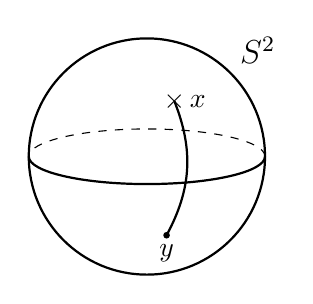
\begin{tikzpicture}
                % Definición de radio y perspectiva
                \def\R{1.5}
                \def\ry{0.35}

                % Esfera (círculo exterior)
                \draw[thick] (0,0) circle (\R);

                % Ecuador (parte trasera discontinua, delantera continua)
                \draw[dashed] (\R,0) arc (0:180:{\R} and {\ry});
                \draw[thick] (-\R,0) arc (180:360:{\R} and {\ry});

                % Etiqueta de la esfera S^2
                \node[above right] at (45:\R) {\large $\bb{S}^2$};

                % Puntos x e y
                \coordinate (X) at (0.35, 0.7);
                \coordinate (Y) at (0.25, -1.0);

                % Dos caminos entre x e y (uno por el frente y otro por detrás)
                % Camino frontal (sólido)
                \draw[thick] (X) to[bend left=25] (Y);

                % Marcas y etiquetas de los puntos
                \node at (X) {$\times$};
                \node[right=2pt] at (X) {$x$};

                \fill (Y) circle (1.2pt);
                \node[below] at (Y) {$y$};
            \end{tikzpicture}
            \caption{Arco entre $x$ e $y$ en $\bb{S}^2$.}
            \label{fig:arcos_s2}
        \end{figure}

        Distinguimos dos casos.
        \begin{itemize}
            \item Si $y\neq -x$, entonces podemos considerar el segmento que une $x$ con $y$ en $\bb{R}^{n+1}$. Este segmento no está contenido en $\bb{S}^n$, pero podemos dividir cada punto de este segmento por su norma para obtener un arco en $\bb{S}^n$ que una $x$ con $y$. Es decir, consideramos:
            \Func{\alpha}{[0,1]}{\bb{S}^n}{t}{\dfrac{(1-t)x + ty}{\|(1-t)x + ty\|}}

            Puesto que $y\neq -x$, se tiene que $(1-t)x + ty \neq 0$ para todo $t\in [0,1]$ y por tanto $\alpha$ está bien definida. Además, $\alpha(0) = x$ y $\alpha(1) = y$.

            \item Si $y=-x$, entonces podemos considerar un punto $z\in \bb{S}^n$ tal que $z\neq x$ y $z\neq y$. Entonces definimos $\alpha_1$ como el arco que une $x$ con $z$ y $\alpha_2$ como el arco que une $z$ con $y$. Entonces $\alpha_1\ast \alpha_2$ es un arco que une $x$ con $y$.
        \end{itemize}
    \end{enumerate}
\end{ejemplo}

\begin{definicion}
    Decimos que un e.t. $X$ es \textbf{arcoconexo} (o \textbf{conexo por arcos}) si para cualesquiera $x,y\in X$ existe un arco en $X$ que une el punto $x$ con el punto $y$.\\

    Si $X$ es un e.t. y $A\subset X$, diremos que $A$ es arcoconexo si $A$ es arcoconexo con la topología inducida de $X$.
\end{definicion}


Como indicamos al principio, la arcoconexión es un concepto más restrictivo que la conexión. Veamos la formalización de esta idea.
\begin{teo}
    Todo espacio topológico arcoconexo es conexo.
    \begin{proof}
        Dado $x_0\in X$ fijo y otro punto $x\in X$ cualquiera, sabemos que existe $\alpha_x:[0,1]\to X$ un arco tal que $\alpha_x(0)=x_0$ y $\alpha_x(1)=x$. En particular, como el intervalo $[0,1]$ es conexo y $\alpha_x$ es continua, entonces se tiene que $\alpha_x([0,1])$ es conexo y podremos escribir 
        \begin{gather*}
            X=\bigcup\limits_{x\in X}\{x\}\subseteq \bigcup\limits_{x\in X} \alpha_x ([0,1])\subseteq X \Rightarrow X = \bigcup\limits_{x\in X}\alpha_x([0,1])
        \end{gather*}
        y además $x_0 \in \bigcap\limits_{x\in X}\alpha_x([0,1])$ por lo que $X$ es conexo por el Teorema~\ref{teo:union_conexos}.
    \end{proof}
\end{teo}

\begin{ejemplo}
    Veamos que la otra implicación no es cierta en general. Para ello consideramos los siguientes conjuntos: 
    \begin{gather*}
        X_0=\{1\}\times [0,1] \hspace{0.5cm}\text{ y } \hspace{0.5cm} X_n = [0,1]\times \left\{\frac{1}{n}\right\},\ n\in \bb{N}
    \end{gather*}

    \begin{figure}[H]
        \centering
        \begin{tikzpicture}[scale=0.8]
            \begin{axis}[
                axis lines=left,
                height=8cm, width=10cm,
                xmin=-0.2, xmax=1.2,
                ymin=0, ymax=1.2,
                xtick={0,1},
                ytick={0,0.5,1},
                yticklabels={$0$,$\tfrac{1}{2}$,$1$},
                grid=major,
                axis x line=middle, % eje X en y=0
                axis y line=middle, % eje Y en x=0
                legend style={at={(1.2,1)},anchor=north east} % posición de la leyenda
            ]
                % Tramos constantes

                \addplot[very thick,blue!60!black] coordinates {(1,0) (1,1)};
                \addlegendentry{$X_0$}

                \addplot[very thick,red!60!black] coordinates {(0,1) (1,1)};
                \addlegendentry{$X_n$}

                \foreach \i in {2,...,100} {
                    \addplot[very thick,red!60!black, forget plot] coordinates {(0,1/\i) (1,1/\i)};
                }

                % Puntoo
                \addplot[only marks,mark=*,green!60!black] coordinates {(0,0)};
                \addlegendentry{$(0,0)$}
            \end{axis}
        \end{tikzpicture}
    \end{figure}

    Llamamos $X=\{(0,0)\}\cup \left(\bigcup\limits_{n\in \bb{N}\cup \{0\}}X_n\right)$ y queremos ver que $X$ es conexo pero no es arcoconexo.\\

    Si tomamos la segunda parte de esta unión, es decir, 
    \begin{gather*}
        Y=\bigcup\limits_{n\in \bb{N}\cup \{0\}}X_n
    \end{gather*}
    tenemos que $Y$ es conexo porque es unión de los $X_n$ que son todos conexos y que intersecan con $X_0$. Entonces, como $Y\subset X \subset \overline{Y}$ tenemos que $X$ es conexo. Veamos sin embargo que $X$ no es arcoconexo.\\

    Para ello vamos a demostrar que si $\alpha:[0,1]\to X$ tal que $\alpha$ es continua con $\alpha(0)=(0,0)$, entonces $\alpha(t)=(0,0)$ para todo $t\in [0,1]$.\\

    Podemos escribir la curva como $\alpha(t) = (x(t), y(t))\in \bb{R}^2$. Como $\alpha(0)=(0,0)$, si tomamos $((-\nicefrac{1}{2}, \nicefrac{1}{2})\times (-\nicefrac{1}{2}, \nicefrac{1}{2})) \cap X$ un abierto que contiene al origen, entonces $\exists \veps > 0$ tal que $\alpha([0,\veps))\subseteq ((-\nicefrac{1}{2}, \nicefrac{1}{2})\times (-\nicefrac{1}{2}, \nicefrac{1}{2})) \cap X$ por ser $\alpha$ continua. Como $y(t)$ es continua y se tiene que $y([0,\veps))\subseteq \{0\}\cup\left(\bigcup\limits_{n>2} \left\{\frac{1}{n}\right\}\right)$. Por el teorema del valor intermedio tenemos que $y([0,\veps)) = \{0\}$ por lo que $\alpha([0,\veps))=\{(0,0)\}$. De esta forma hemos probado que no hay ningún arco que conecte $(0,0)$ con un punto distinto (el único arco es el constante).
\end{ejemplo}

\begin{teo}
    Si $A\subseteq \bb{R}^n$ es estrellado, entonces $A$ es arcoconexo.
    \begin{proof}
        Como $A$ es estrellado existe un $x_0\in A$ tal que para cualquier $x\in A$, el segmento que los une, $(1-t)x + tx_0\in A$ para todo $t\in [0,1]$ y entonces $\alpha(t)=(1-t)x+tx_0$ es una curva continua uniendo $x$ con $x_0$. Dados dos puntos cualesquiera $x,y \in A$ se tiene que $\alpha_x\ast \tilde{\alpha}_y$ es una curva continua que une $x$ con $y$.
    \end{proof}
\end{teo}

\begin{coro}
    Cualquier conjunto $A$ de $\bb{R}^n$ convexo es arcoconexo. En particular, las bolas abiertas y las bolas cerradas de $\bb{R}^n$ son arcoconexas.
\end{coro}

\begin{coro}
    En $\bb{R}$ coinciden los conjuntos conexos y arcoconexos (son solo los intervalos).
\end{coro}

\begin{teo}
    La imagen mediante una aplicación continua de un arcoconexo es un arcoconexo. En particular, ser arcoconexo es una propiedad topológica, es decir, se conserva por homeomorfismos.
    \begin{proof}
        Sea $f$ la aplicación continua y consideramos $x,y\in f(X)$ cualesquiera. Entonces existen $x_0,y_0\in X$ tal que $f(x_0)=x$ y $f(y_0) = y$. Por ser $X$ arcoconexo tenemos que existe un arco $\alpha:[0,1]\to X$ con $\alpha(0)=x_0$ y $\alpha(1)=y_0$. Entonces tenemos que $f\circ \alpha: [0,1]\to f(X)$ es continua y además
        \begin{gather*}
            (f\circ \alpha)(0) = f(x_0) = x \ \ \ \text{ y } \ \ \ (f\circ\alpha)(1) = f(y_0) = y
        \end{gather*}
        y tenemos por tanto que $(f\circ \alpha)$ es un arco que une $x$ con $y$. Tenemos entonces que para cualesquiera dos puntos $x,y\in f(X)$ existe un arco que los une luego $f(X)$ es arcoconexo.
    \end{proof}
\end{teo}

\begin{teo}
    Sean $X$ un e.t. y $\{A_i\}_{i\in I}$ una familia de arcoconexos de $X$. Si $\bigcap\limits_{i\in I}A_i \neq \emptyset$, entones $\bigcup\limits_{i\in I}A_i$ es arcoconexo.
\end{teo}

\begin{observacion}
    Hay resultados de conexión que no son ciertos para arcoconexión. Por ejemplo, si en un e.t. $X$ se tiene que $A\subseteq X$ es arcoconexo podría ocurrir que si $A\subseteq B \subseteq \overline{A}$, se diera que $B$ no sea arcoconexo (como en el ejemplo anterior).
\end{observacion}

\begin{ejemplo}
    Veamos que $\bb{S}^n = \{x\in \bb{R}^{n+1} : |x| = 1\}$ es arcoconexo. Podemos hacerlo sabiendo que $\bb{S}^n\setminus \{N\}$, con $N=(0,\dots,0,1)$ es homeomorfo a $\bb{R}^n$ que es arcoconexo por lo que $\bb{S}^n \setminus\{N\}$ es arcoconexo. Análogamente, $\bb{S}^n \setminus\{S\}$ con $S=(0,\dots,0,-1)$ es arcoconexo y podemos escribir
    \begin{gather*}
        \bb{S}^n = (\bb{S}^n \setminus\{N\}) \cup (\bb{S}^n \setminus\{S\})
    \end{gather*}
    por lo que $\bb{S}^n$ es unión de arcoconexos con puntos en común, luego es arcoconexo.
\end{ejemplo}

\begin{teo}
    Sean $X,Y$ e.t., entonces $X\times Y$ es arcoconexo (con la topología producto) si y solo si $X$ e $Y$ son arcoconexos.
\end{teo}

\begin{teo}
    Dado un e.t. $X$, se tiene que $X$ es arcoconexo si y solo si $X$ es conexo y todo punto $x\in X$ tiene un entorno suyo arcoconexo.

    \begin{proof}\
        \begin{itemize}
            \item[$\Rightarrow$)] Hemos visto que si $X$ es arcoconexo, entonces $X$ es conexo. Además, $X$ es entorno de cualquier punto suyo luego todo punto tiene un entorno arcoconexo.
            \item[$\Leftarrow$)] Elegimos un $x\in X$ fijo y definimos $A = \{y\in X : \exists \alpha_y \text{ arco uniendo $x$ con $y$ }\}$
            
            Como $x\in A$ tenemos que $A\neq \emptyset$. Si probamos que $A$ es abierto y cerrado, entonces como $X$ es conexo tendremos que $A=X$, es decir podremos unir $x$ con cualquier otro punto $y\in X$.\\

            Veamos que $A$ es abierto. Tomamos $z\in A$ y queremos demostrar que $\exists U$ entorno de $z$ tal que $U\subseteq A$. Por hipótesis sabemos que existe un entorno $U$ arcoconexo de $z$. Entonces dado $u\in U$ existe un arco $\alpha_u$ que une $z$ con $u$. Por otro lado, como $z\in A$, entonces existe un arco $\beta_z$ que une $x$ con $z$. Tendremos entonces que $\beta_z\ast\alpha_u$ es un arco que une $x$ con $u$ y por definción tendremos $u\in A$, luego $U\subseteq A$.\\
            
            Nos queda ver que $A$ es cerrado. Tomamos para ello $z\in \overline{A}$. Por hipótesis existe un entorno $U$ de $z$ arcoconexo. Por ser $U$ entorno de $z$ y $z\in \overline{A}$ necesariamente $U\cap A \neq \emptyset$ por lo que existe al menos un $u\in U \cap A$. Como $u\in A$ existe un arco $\alpha_u$ que une $x$ con $u$ y como $u\in U$ existe también un arco $\beta_u$ que une $u$ con $z$ y tendríamos que $\alpha_u\ast\beta_u$ es un arco uniendo $x$ con $z$ llegando a que $z\in A$. Tendríamos $\overline{A}\subseteq A$ y como la otra inclusión se da siempre, tendremos que $A$ coincide con su adherencia, por lo que es cerrado.
        \end{itemize}
    \end{proof}
\end{teo}

\begin{definicion}
    Dados un e.t. $X$ y un punto $x_0\in X$, llamamos \textbf{componente arcoconexa} de $x_0$ al mayor arcoconexo en $X$ que contiene a $x_0$.
\end{definicion}

\begin{teo}
    Las componentes arcoconexas de un e.t. $X$ forman una partición de $X$ en subconjuntos arcoconexos de $X$ maximales.
\end{teo}

\begin{ejemplo} En el ejemplo que ya se trabajó se puede ver que el conjunto $X$ que era

    \begin{figure}[H]
        \centering
        \begin{tikzpicture}[scale=0.8]
            \begin{axis}[
                axis lines=left,
                height=8cm, width=10cm,
                xmin=-0.2, xmax=1.2,
                ymin=0, ymax=1.2,
                xtick={0,1},
                ytick={0,0.5,1},
                yticklabels={$0$,$\tfrac{1}{2}$,$1$},
                grid=major,
                axis x line=middle, % eje X en y=0
                axis y line=middle, % eje Y en x=0
                legend style={at={(1.2,1)},anchor=north east} % posición de la leyenda
            ]
                % Tramos constantes

                \addplot[very thick,blue!60!black] coordinates {(1,0) (1,1)};
                \addlegendentry{$X_0$}

                \addplot[very thick,red!60!black] coordinates {(0,1) (1,1)};
                \addlegendentry{$X_n$}

                \foreach \i in {2,...,100} {
                    \addplot[very thick,red!60!black, forget plot] coordinates {(0,1/\i) (1,1/\i)};
                }

                % Puntoo
                \addplot[only marks,mark=*,green!60!black] coordinates {(0,0)};
                \addlegendentry{$(0,0)$}
            \end{axis}
        \end{tikzpicture}
    \end{figure}

    tiene dos componentes arcoconexas: $\{(0,0)\}$ , $\bigcup\limits_{u\in \bb{N}\cup\{0\}}X_n$
\end{ejemplo}

